\chapter{Calibration Of A Sensor Network}


The use of sensor networks for pollution monitoring has given the freedom to set up a monitoring system at residences, offices, or even at schools. One of the main drawbacks of this is to identify the accuracy of the data collected from these low-cost sensors compared to the reference monitoring system. If the sensor system gives values that are different from the reference system then it brings into question the advantages of this technology. This issue can be resolved through calibration which will reduce the uncertainty in data and make the output more accurate. 
%The reference system are the pollution monitoring devices that are developed with a defined standard for a specific criteria pollutant[s] and has completed a rigorous testing and analysis protocol \cite{Hall2014}.
\par 

Calibration can be defined as an act of evaluating and adjusting the precision and accuracy of measurement equipment \cite{miskell2018solution}. If the measured output from the sensor is not equal to the output from a reference system then it shows that there is a need for calibration. In general, all electronic instruments are calibrated according to given set conditions and acquire a certification of calibration before being sold. Even then the measured value might not reach the specified accuracy as the condition in the environment where it was calibrated changes, leaving the user with values that give poor information. This issue was taken up and explored by many researchers around the globe. During the 2013 Air Sensor Workshop, the US Environmental Protection Agency (EPA) suggested the three "straw-man calibration" approaches to improve the usability of uncertain data \cite{Williams2013}. 

The first approach is \lq{signal-based calibration}\rq technique that requires the data from the reference station to be broadcast to the local station where the sensor is located and which will receive this data and perform a single point calibration of its response. This approach is feasible if the sensor is equipped with the data collection and can process automatic calibration. 


The next approach for calibration is called \lq{direct sensor calibration}\rq that involves placing the sensor in a chamber in which a known concentration of pollutant is present and the response is observed. As the concentration of the pollutant is known, the output curve can be compared with it and calibrated accordingly. This is the most common method used for calibration in laboratories. Another way of approaching \lq{direct sensor calibration}\rq is by inspecting the pre-defined response given by the manufacturer and determining the sensor response to a given concentration. In either case the calibration requires equipment and skills to introduce an accurate concentration value.


The last approach is \lq{secondary data normalization}\rq in which the concentration values of the pollutant from the low-cost sensor are normalized in accordance with the federal reference method (FRM) or federal equivalent method (FEM) analyzers. This approach is cost-effective when compared to the other techniques and is less complex. This can be achieved by the use of a linear mathematical equation model that will convert the non-calibrated data into data of an acceptable form. The linear relationship equation $ y = mx + c $ where $ m $ is the slope and $ c $ is the intercept of the sensor raw data is compared with analyzer data and a relationship pattern is established from this. The drawback of this approach is that the sensor does not always give a linear response and thus not applicable for all the curves. Even though these Straw-Man approaches were defined it can be hard to implement any of them in practice. 

By the end of the workshop, it was widely agreed by the researchers that developing a software tool that can guide researchers through calibration procedures. By Fall 2016 the EPA developed a \lq{Macro Analysis Tool}\rq (MAT) that performs comparisons of low-cost sensor data with the reference system data and is included in \lq{Air Sensor Toolbox}\rq \cite{airsensortoolbox}.  In our research project, we replicated the MAT tool in the form of a webpage so that the user can upload data and recieve back the calibration curve. In the next section, we explain the working of the MAT tool and the procedures we followed for data calibration in detail.


\section{Macro Analysis Tool - MAT}


The development of the MAT supports researchers in calibrating sensor data. This is an Excel-based, user-friendly macro tool that compares sensor data with reference data \cite{National2017} even if measurements weren’t recorded at precisely the same time, or were collected at different time sampling intervals, such as 1-minute versus 5-minute intervals \cite{mattool}. 

The MAT tool allows the user to insert the collected data and timestamps from both the reference system and low-cost sensor system into their respective pages of Excel sheets.
After the data are provided the details of pollutants, time interval, measurement units and data completeness (amount of usable data obtained) are added in the control panel page of the MAT as shown in Figure \ref{controlpanel}. Once these are filled out the user clicks the \lq{RUN}\rq button to perform the linear regression procedures.


\begin{figure}[h]
  \begin{center}
  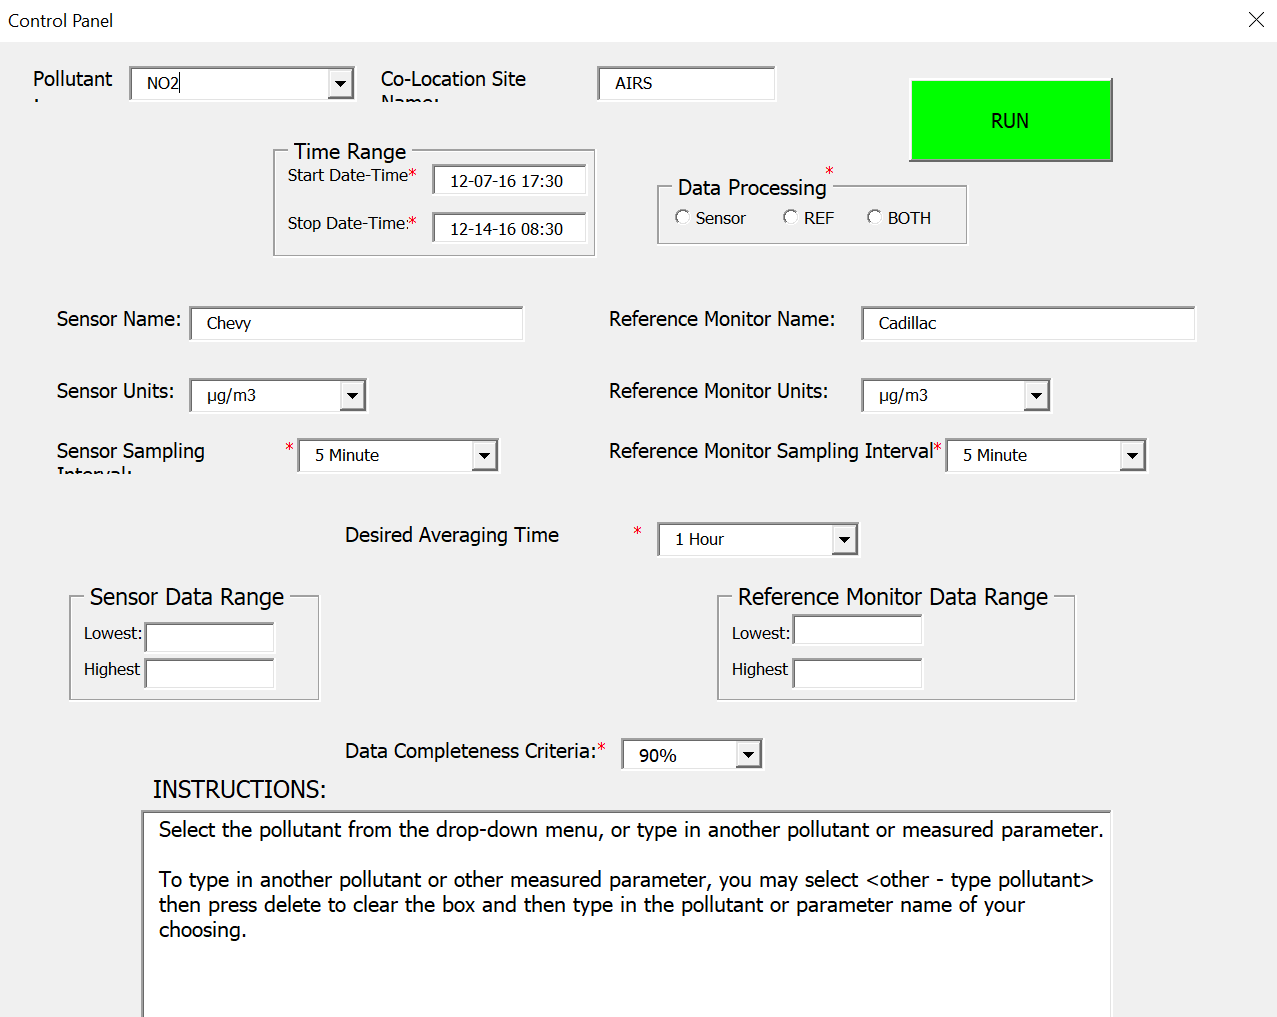
\includegraphics[scale=0.51]{./images/figure43.png}
  \end{center}
  \caption{Control panel of MAT tool  \cite{National2017}}
  \label{controlpanel}
  \hspace{1 cm}
\end{figure}








An example of the output page of the MAT is as shown in Figure \ref{MAT} in which the two sets of data being compared as per the control panel setting in the tool \cite{National2017}.
This output page gives a statistical comparison of the two different data sets. From this page it can be seen that the date and time stamps are averaged to a single value for both systems. There is another column in the sheet which lists the invalid data points and gives the total number of non validated data points during the observation time. These non validated data points occur due to either data issues from the instrument or issues in reading values by MAT or unacceptable ranges specified by the user.

\begin{figure}[h]
    \begin{center}
    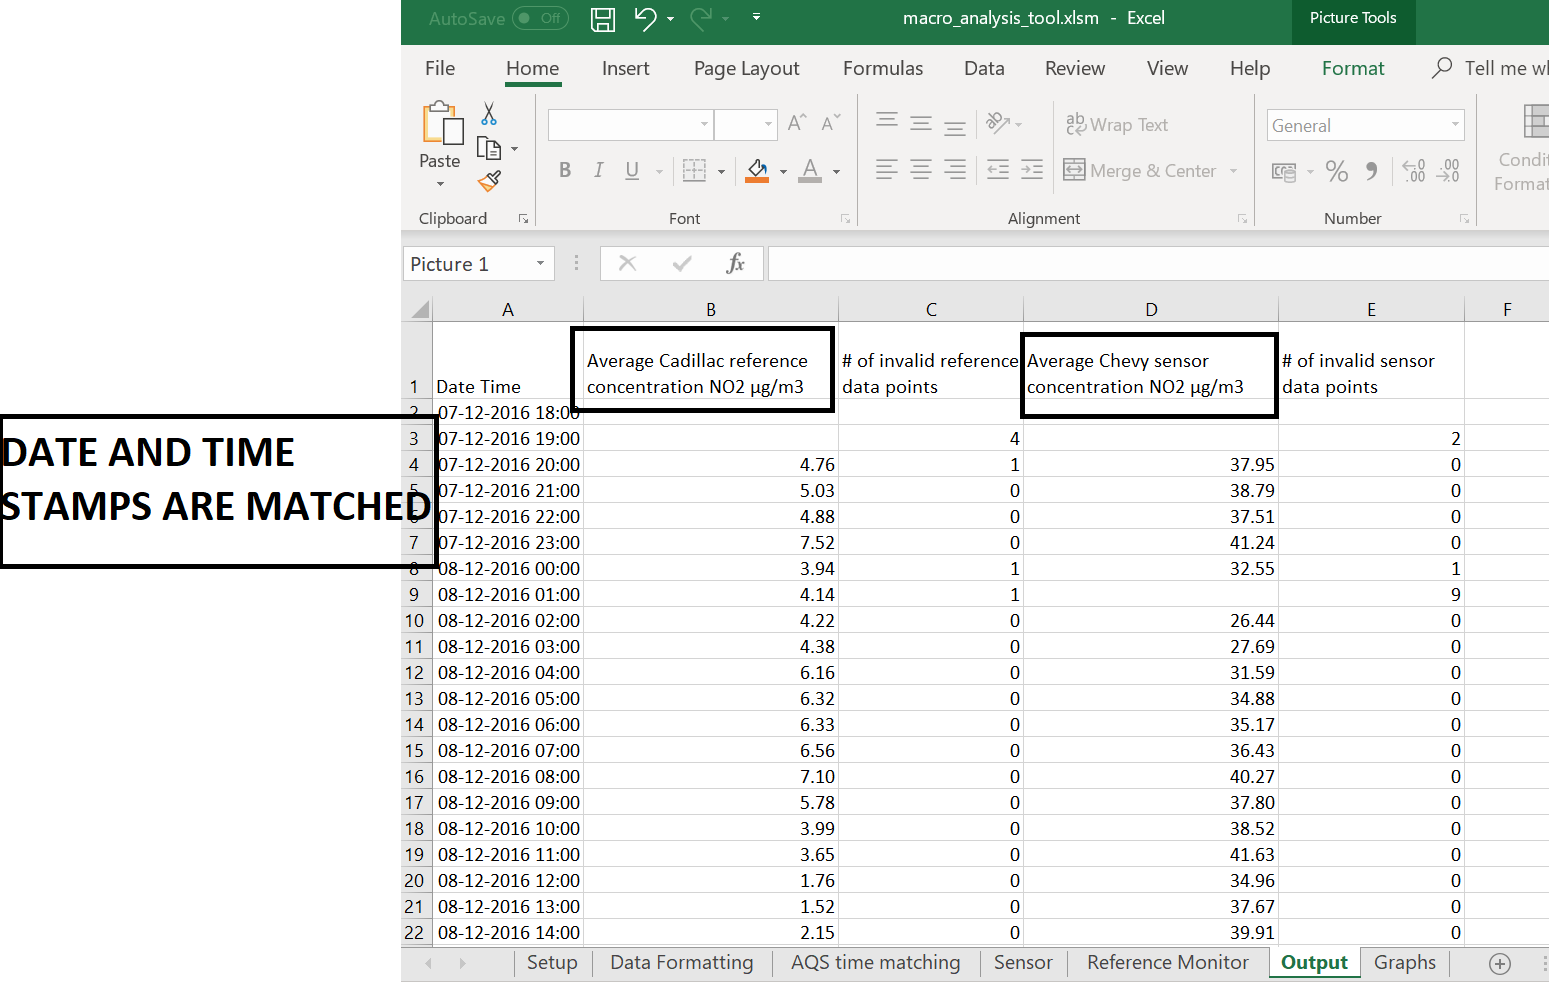
\includegraphics[scale=0.55]{./images/figure6.png}
    \end{center}
    \caption{Output page of Macro Analysis Tool \cite{MATEXCEL}}
    \label{MAT}
    \hspace{1 cm}
  \end{figure}

\par


The next output page provided by the tool is the linear regression result which is a correlation graph between the reference monitor and the sensor data. An example of the output page is shown in Figure \ref{cor}. The graph drawn is a scatter plot and a slope-intercept line will be drawn through the data points. This line describes the average behaviour of the sensor data on the vertical axis compared with the reference data on the horizontal axis \cite{National2017}. The fit of the graph shows the similarity in sensor measurements when compared with the reference instrument, on average. 

\hspace{1 cm}
\begin{figure}[h]
    \begin{center}
    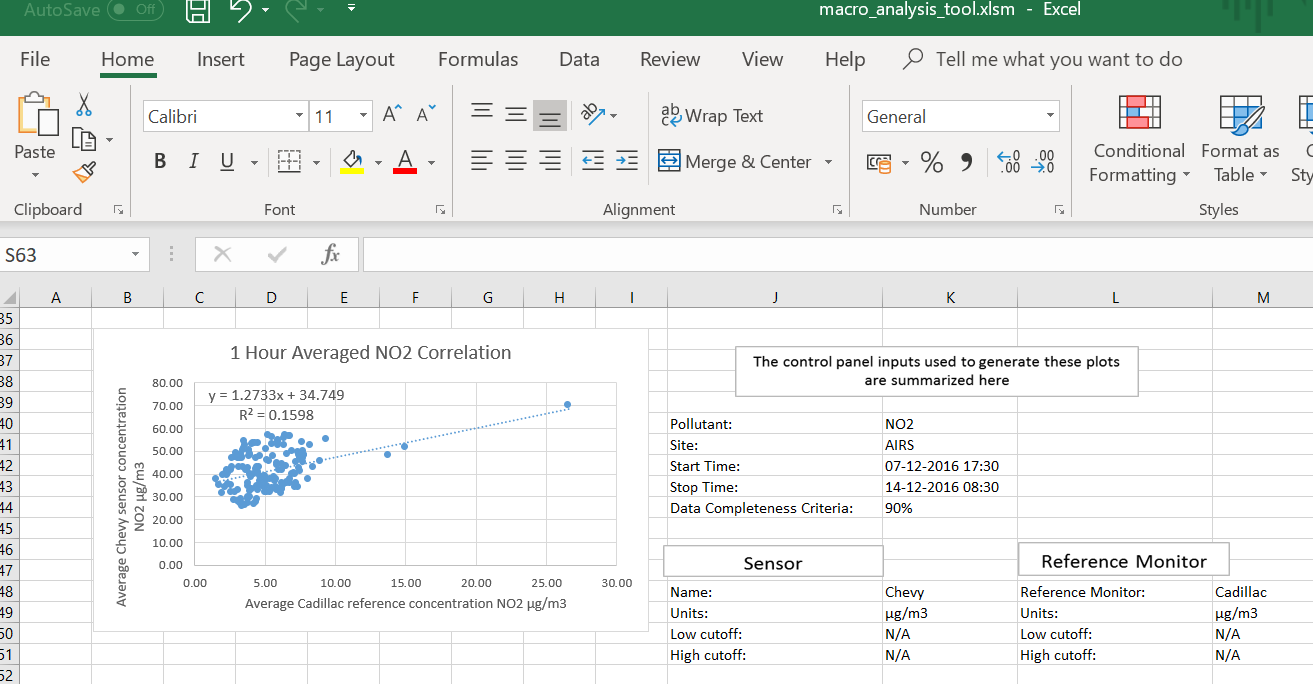
\includegraphics[scale=0.50]{./images/figure7.png}
    \end{center}
    \caption{Correlation Graph}
    \label{cor}
  \end{figure}
 
The tool also generates a correlation coefficient (R-Squared, $R^2 $) that indicated how close the values are to the slope-intercept line. The $R^2 $ ranges from 0 to 1 and the closer $R^2$ is to 1, the stronger the agreement between the sensor and the reference data \cite{Williams2018}. Along with these outputs, the tool also generates a time series output graph which shows the concentration of pollutants for both systems as shown in Figure \ref{time}

\begin{figure}[h]
    \begin{center}
    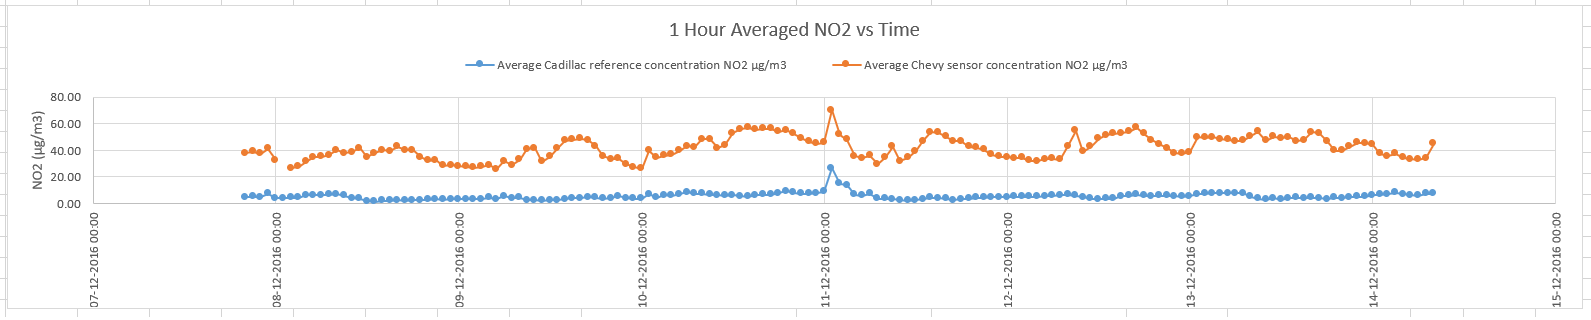
\includegraphics[scale=0.55]{./images/figure8.png}
    \end{center}
    \caption{Time-Series Graph}
    \label{time}
  \end{figure}

From the time-series graph in Figure \ref{time} it can be seen how the closely value from the two systems are related.
Having included all of this functionality in the MAT gives a workable solution for the calibration issue. The development of the tool was a year-long project for EPA with community groups (Clean Air
Carolina) and  one tribal nation (Eastern Band of Cherokee Indians).





%An year later the development of the \lq{Air Sensor Toolbox}\rq by the Environmental Protection Agency (EPA) \cite{Williams2014} which introduced \lq{Macro Analysis Tool}\rq (MAT) for performing comparisons of air sensor data with reference data and interpreting the results \cite{airsensorguidebook}.The EPA also developed a \lq{Air Sensor Guidebook}\rq that could assist those interested in air quality measurement with low-cost sensors.

\section{Calibration Procedure}


The calibration procedure we followed is from the \lq{Air Sensor Toolbox}\rq  guidelines for researchers, citizens, scientists, and developers who are working with low-cost sensors and their calibration to get more insight on air quality \cite{airsensortoolbox}. The Air Sensor Toolbox \cite{airsensorguidebook} provides a three-step procedure for calibrating a sensor:
\begin{enumerate}
    \item Comparing the data from the low-cost sensor with a reference instrument.
    
The data collected from the sensor system should be compared with the data from an already calibrated system that is placed by the local authority. This type of comparison is called  \lq{collocation}\rq and to collocate, we need to find out where the reference system is placed and get access to the data from the reference system. Once we have access to the data collected from both the reference system and the low-cost sensor system, then the data can be downloaded in the desired format.

    \item Creating a calibration curve with the help of the Macro Analysis Tool (MAT).

The relationship between the response of an analytical instrument to the concentration or amount of an analyte introduced into a known instrument is referred to as the “calibration curve” \cite{Epa2010} and is obtained by linear regression. Linear regression establishes a relationship between two variables, the independent variable which will be on the $x$ axis and the dependent variable in the $y$ axis by drawing a best fit straight line \cite{regression}. The MAT tool by EPA is used for finding the calibration curve and will give an error function as output. This error function is an equation which can be used for calibrating the sensor.
    \item Repeating the calibration periodically.

    This procedure of calibration should be done periodically as the performance of instruments changes.It is expected that there will be changes in the best fit equation over time and this should be noted so as to get accurate values.
\end{enumerate} 


\iffalse

\section{Linear Regression}

[COMMENT:  Not sure whether this section to be added or not]

Calibration can be done through different statistical methods and the most popular approach is Linear Regression method. In statistics, the term regression is used to describe a group of methods that summarize the degree of association between one variable (or set of variables) and another variable (or set of variables) \cite{Burke}. Linear Regression establishes relationship between two variables one is the independent variable which will be on the $x$ axis and the dependent variable in the $y$ axis by drawing a straight line.
If there are many observations and is plotted as a scatter plot then a line called as regression line as in the figure \ref{LRM} could be drawn through it by Least Square method. 


\begin{figure}[h]
    \begin{center}
    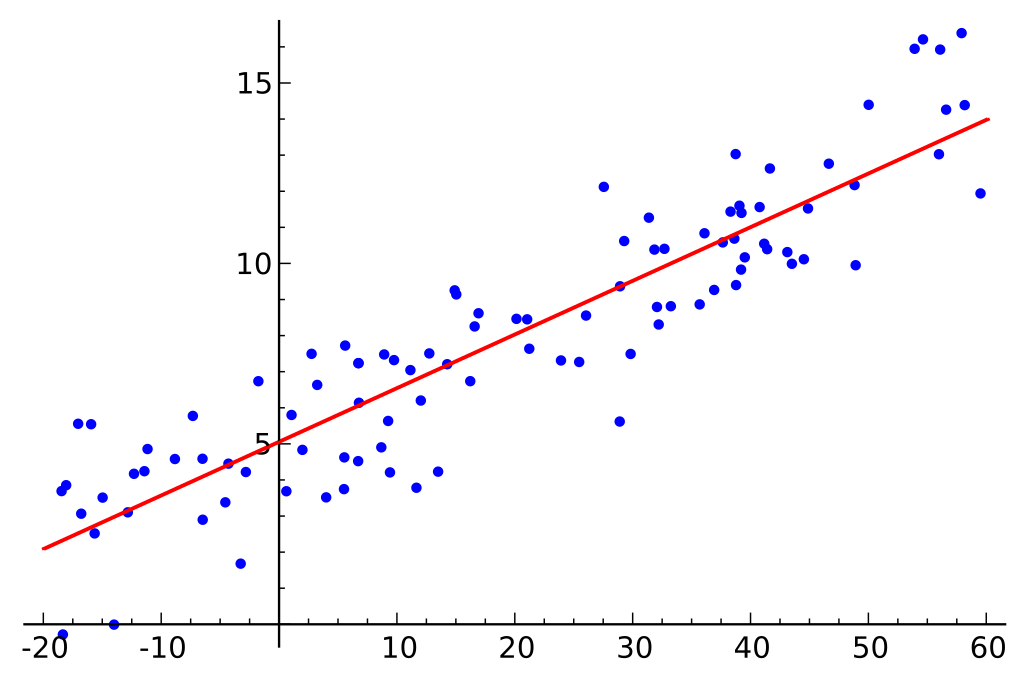
\includegraphics[scale=0.25]{./images/figure9.png} 
    \end{center}
    \caption{Linear Regression Model \cite{regression}}
    \label{LRM}
  \end{figure}
  The method of Least Squares is a procedure to determine the best fit line to data\cite{S.Miller1992} by minimizing the errors between the observed value and the actual value. This method considers that, for each value of $x$, there is a sub-population of $y$ values normally distributed, that the means of all the sub-populations of $y$ lie on the same straight line and all the sub-populations of $y$ values have equal variances \cite{Almeida2002} \cite{daniel2018biostatistics}.
  The line drawn will have a slope $m$ and is given by the formula
\begin{center}

    
             {\large  $ m = \frac{\sum_{i}[(x_i-\bar{x})(y_i-\bar{y})]}{[ \sum_{i}(x_i-\bar{x})^2 ]}$} \cite{Stone2001} \cite{Arsova2009} \cite{Burke}


\end{center}
where $m$ is the slope, $x_i$ and $y_i$ are the reference and observed data values, $\bar{x}$ and $\bar{y}$ are the mean values of the data. The mean values will act as the centroid of the regression line and it has to pass through these points.
The intercept equation $c$ is

\begin{center}
 
    { $ C = \bar{y}-m\bar{x}$} \cite{Stone2001} \cite{Harvey2016}

\end{center}

On getting the slope and intercept value the equation of line can be found. Once the Regression line is drawn, to find out how much the data is scattered and to what extend, correlation coefficient ($R^2$) is used. In other words $R^2$ gives the measure of  degree to which the values of x and y are linearly correlated \cite{Stone2001}. The equation for finding the regression value is

\begin{center}

    {\large $R^2 = \frac{\sum_i[(x_i-\bar x)(y_i-\bar y)]}{\sqrt{[\sum_i(x_i-\bar x)^2[\sum_i(y_i-\bar y)^2]]}}$ } \cite{Stone2001}

\end{center}
The range of value for $R^2$ is between 0 to 1 and closer the value is to 1, the stronger the correlation between the two data.
All these equation can be easily calculated with the help of Excel and thus all these equations are integrated to the MAT tool.

\fi

\section{Framework}

We believe that the MAT tool provides an efficient method for a calibration procedure for a low-cost sensor system. In our work, we have replicated the MAT tool into an IoT platform. This platform gives users the ability to input the values collected from the reference system and any low-cost sensor system. Our implementation makes the calibration procedure possible for any internet connected sensor system, so does not require the Excel software product.

\begin{figure}[h]
  \begin{center}
  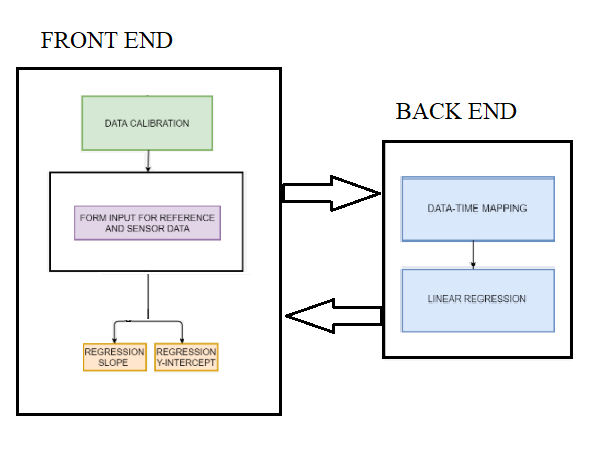
\includegraphics[scale=1.09]{./images/figure32.png} 
  \end{center}
  \caption{Framework of Calibration tool}
  \label{frame}
\end{figure}

Data is uploaded to the online platform in a comma-separated values (csv) file format along with their date and time. After the required data is uploaded the linear analysis takes place and the regression slope and y- intercept is provided as the output. This output regression equation is then used as the calibration equation and applied to the system. The framework of the calibration tool is shown in Figure \ref{frame}. This tool can be accessed from anywhere in the world. The main reason for building such a tool was to have it easily accessed by any networked IoT device.


%This tool has followed the same calibration procedure as that of the MAT tool in which the data from both the system is compared and generates a calibration curve. The calibration equation which is the output is used in the system to obtain the calibrated value.

\section{Summary}

In this chapter, we have discussed how we can establish with the accuracy of our low- cost sensor system. We have discussed the MAT used for calibrating the measured data from the system and we have implemented an IoT version of the tool. In the next chapter, we will discuss the results obtained from our system and its comparison with the reference system in Prince George.


